In questo primo esperimento si vuole valutare il \textbf{clipping} del segnale di uscita, dovuto alla limitazione della massima tensione di uscita dell'operazionale. Il circuito è rappresentato in Figura \ref{fig:Circuito1}. Sono stati utilizzati i seguenti componenti:
\begin{itemize}
    \item Amplificatore operazionale 741, codice LM741CN
    \item Resistenza di ingresso $R_1$, da 0.25W e valore da calcolare
    \item Resistenza di uscita $R_2$, da 0.25W e valore da calcolare
\end{itemize}
\begin{figure}[H]
    \centering
    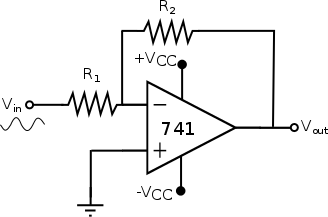
\includegraphics[width=0.7\linewidth]{images/Circuit1.png}
    \caption{schema circuito}
    \label{fig:Circuito1}
\end{figure}
Il circuito è alimentato dalla tensione duale: $\pm V_{CC}=\pm 10V$. I pinout dell'integrato LM741CN sono stati ricavati dal datasheet, riportati in Figura \ref{fig:IC741}
\begin{figure}[H]
    \centering
    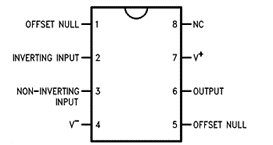
\includegraphics[width=0.5\linewidth]{images/IC741.png}
    \caption{layout dell'integrato LM741CB }
    \label{fig:IC741}
\end{figure}
Dall'analisi del datasheet inoltre si ricava che la tensione massima di alimentazione è $\pm 18V$.
\subsection{Definizione dei valori di $R_1,R_2$ - prelab}
Il circuito amplificatore, riportato in Figura \ref{fig:Circuito1} è in configurazione invertente, di conseguenza il guadagno è
\begin{equation}
    G_1=-\frac{R_2}{R_1}
\end{equation}
Il cui valore, espresso in decibel, deve essere, come da consegna, $23.5dB$
\begin{equation}
    G_1\big|_{dB} = 20log_{10}(|G_1|) = 23.5dB
\end{equation}
Da cui si può ricavare il rapporto tra $R_1$ e $R_2$ pari a 
\begin{equation}
    \frac{R_2}{R_1}=10^{\frac{23.5}{20}}=15
\end{equation}
Si sono quindi scelti i seguenti valori per le resistenze $R_1$ e $R_2$:
\begin{itemize}
    \item $R_1=1\text{k}\Omega$
    \item $R_2=15\text{k}\Omega$
\end{itemize}
\subsection{Valutazione del datasheet - prelab}
Sulla base delle informazioni contenute nel datasheet, si è stimata la massima tensione raggiungibile dall'uscita del circuito a fronte di una alimentazione $\pm V_{CC}=\pm 10V$ 
\begin{equation*}
    V_{{out}_{\text{MAX}}} = \pm 9.33 V
\end{equation*}
NB: nel datasheet non vengono riportati i valori relativi all'alimentazione usata, il valore di tensione massimo è stato stimato utilizzando i dati a disposizione applicando una proporzione.
\subsection{Layout del circuito - prelab}\label{sec:Pre1}
Utilizzando il software Tinkercad è stato possibile rappresentare un possibile layout del circuito su breadboard, visibile in Figura \ref{fig:BreadBoard1}
\begin{figure}[H]
    \centering
    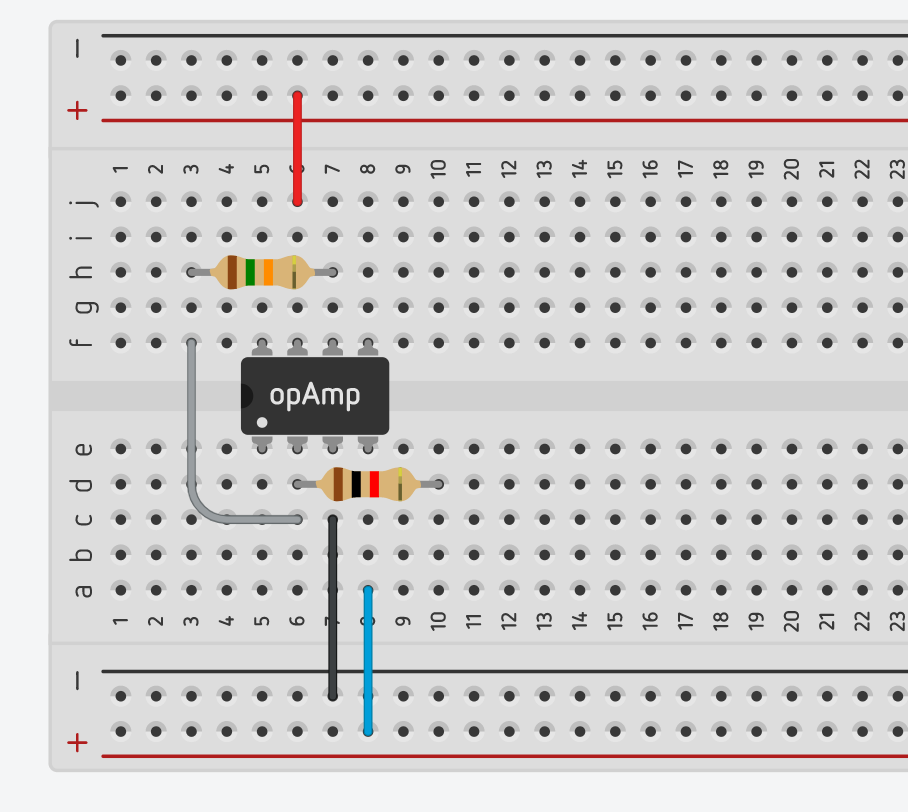
\includegraphics[width=0.4\linewidth]{images/BreadBoard1.png}
    \caption{Circuito su breadboard}
    \label{fig:BreadBoard1}
\end{figure}
\subsection{Assemblaggi e settaggi}
Una volta montato il circuito in Figura \ref{fig:Circuito1} secondo il layout definito in fase di prelab al punto \ref{sec:Pre1}, è stata collegata l'alimentazione duale $\pm V_{CC}=\pm10V$, come in Figura \ref{fig:Alimentazione1}. \\
\begin{figure}[H]
    \centering
    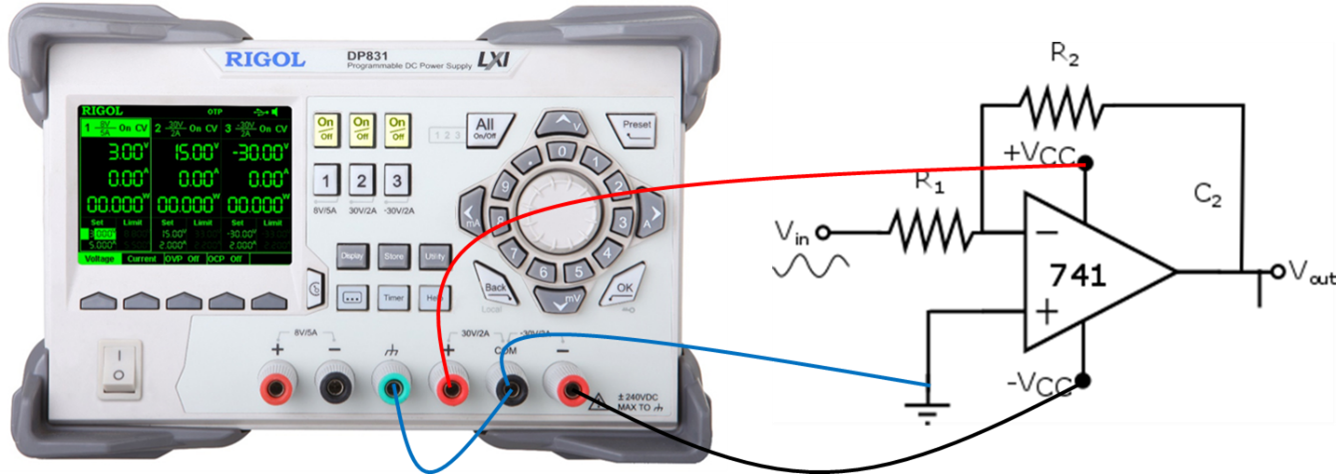
\includegraphics[width=0.7\linewidth]{images/LabCircuit1.png}
    \caption{Schema di collegamento dell'alimentazione}
    \label{fig:Alimentazione1}
\end{figure}
In seguito è stato collegato la "T" BNC all’uscita del generatore di funzione; una delle terminazioni della "T" al canale 1 dell'oscilloscopio e l'altra al circuito. Infine l'uscita del circuito è stata connessa  al canale 2 dell' oscilloscopio. Come si vede in Figura \ref{fig:LabCircuit1}
\begin{figure}[H]
    \centering
    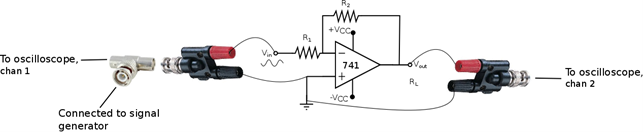
\includegraphics[width=0.7\linewidth]{images/LabCircuit1.1.png}
    \caption{Schema di collegamento dei segnali e oscilloscopio}
    \label{fig:LabCircuit1}
\end{figure}
Il generatore di forma d'onda è stato impostato con il seguente segnale:
\begin{itemize}
    \item Forma d'onda: quadra
    \item Ampiezza: $100mV$ picco-picco
    \item Frequenza: $300Hz$
    \item Duty cycle: 50\%
\end{itemize}
Dopo aver verificato la corretta connessione dei componenti del circuito, la giusta regolazione delle impedenze degli ingressi dei canali dell'oscilloscopio e dell'uscita del generatore di funzione; è stato acceso il generatore di alimentazione.
\clearpage
\subsection{Risultati}
L'oscilloscopio è stato impostato in modo da visualizzare simultaneamente i segnali $V_{in}$ e $V_{out}$, come si vede in Figura \ref{fig:Ris1}
\begin{figure}[H]
    \centering
    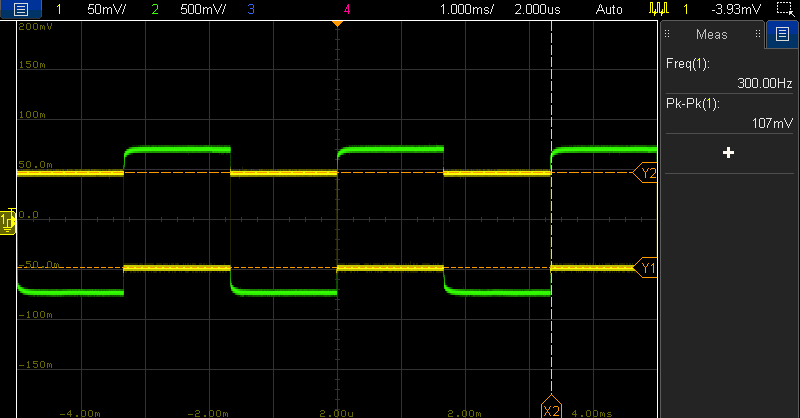
\includegraphics[width=0.7\linewidth]{images/Ris1.png}
    \caption{Forme d'onda catturate dall' oscilloscopio (le scale di tensioni dei due canali sono diverse)}
    \label{fig:Ris1}
\end{figure}
Successivamente sono stati misurati i parametri presentati in tabella, utilizzando le funzioni integrate e i cursori.
\begin{table}[H]
    \centering
    \begin{tabular}{|c|c|}
        \hline
        Frequenza del segnale di ingresso & 300.0Hz \\\hline
        Ampiezza picco-picco del segnale di ingresso &  $94.5mV$ \\\hline
        Ampiezza picco-picco del segnale di uscita & $1.41V$ \\\hline
        Guadagno di tensione dell'amplificatore & $23.47dB$
        \\\hline
    \end{tabular}
    \caption{Risultati misure oscilloscopio}
    \label{tab:Ris1}
\end{table}
NB: il guadagno di tensione è stato calcolato con $20\log_{10}{\frac{1.41V}{94.5mV}}=23.47dB$
\subsubsection{Tensione di clipping}
Nella seconda parte del primo esperimento si vuole misurare la tensione di clipping del segnale in uscita. Si è impostato il generatore di forma d'onda come segue
\begin{itemize}
    \item Forma d'onda: sinusoidale
    \item Ampiezza iniziale: $100mV$ picco-picco
    \item Frequenza: 300Hz
\end{itemize}
Si è poi aumentata l'ampiezza picco-picco del segnale di ingresso fino a quando si è osservato il clipping della tensione di uscita. Esso si è verificato alla tensione di ingresso di $1.22V$.\\
Come possiamo vedere dalla Figura \ref{fig:Ris1.1} la semionda negativa assume la distorsione tipica di un segnale clippato.
\begin{figure}[H]
    \centering
    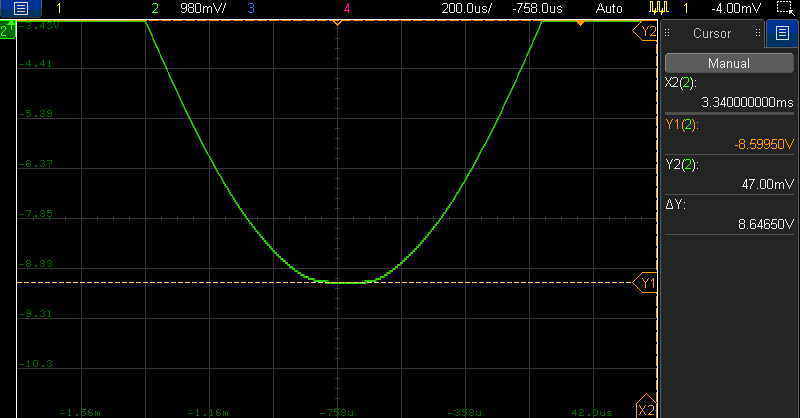
\includegraphics[width=0.7\linewidth]{images/Ris1.1.png}
    \caption{Segnale di uscita clippato}
    \label{fig:Ris1.1}
\end{figure}
In questa condizione di misura abbiamo preso nota dei seguenti parametri:
\begin{table}[H]
    \centering
    \begin{tabular}{|c|c|}
    \hline
    Tensione di ingresso a cui si instaura il clipping del segnale in uscita & $1.22V$ \\\hline
    Tensione di clipping del segnale di uscita, semionda positiva & $8.637V$ \\\hline
    Tensione di clipping del segnale di uscita, semionda negativa & $-8.600V$ \\\hline
    Differenza tra la tensione di clipping positiva e alimentazione positiva & $8.637V-10V=-1.363V$ \\\hline
    Differenza tra la tensione di clipping negativa e alimentazione negativa & $-8.6-(-10V)=1.4V$ \\\hline
    \end{tabular}
    \caption{Risultati delle misurazioni del segnale in clipping}
    \label{tab:Ris1.1}
\end{table}